\section{Cross-Family Case Divergence and Supplementary Ablations}
\label{app:archive}

\begin{figure*}[!t]
\centering
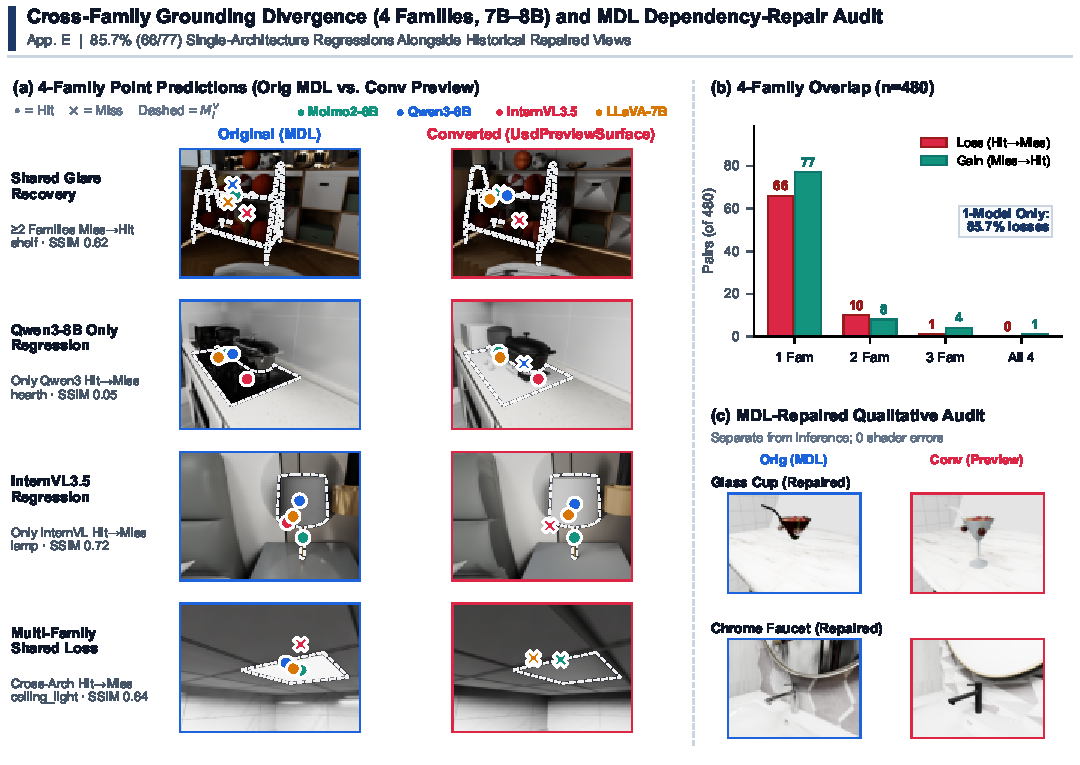
\includegraphics[width=0.92\textwidth]{app_fig4_multifamily_gallery.pdf}
\caption{\textbf{Cross-family localization divergence across 7B--8B architectures and repaired \textsc{MDL} audit.}
\emph{(a)} Representative target-centered captures across the four $\ge$7B families (\textsc{Molmo2-8B}, \textsc{Qwen3-VL-8B}, \textsc{InternVL3.5-8B-HF}, and \textsc{LLaVA-NeXT-Mistral-7B}) comparing \original{} (\textsc{MDL}) against \converted{} (\usdps{}) with simulator mask outlines $M_i^v$: shared glare recovery, architecture-unique regressions, and multi-family failures.
\emph{(b)} Distribution of how many architectures share each regression or gain across all 480 pairs ($66/77 = 85.7\%$ of regressions occur in one model only).
\emph{(c)} Representative pairs rendered after \textsc{MDL} asset dependency repair.}
\label{fig:app-multifamily}
\end{figure*}

\subsection{Architecture-specific localization failures in the 30-scene suite}
Across the four $\ge$7B families evaluated on all 480 captures, $77/480$ pairs experience at least one conversion regression (\emph{Loss}), yet \textbf{$66/77$ ($85.7\%$) of those regressions occur in only a single architecture}, $10/77$ ($13.0\%$) affect two architectures, $1/77$ ($1.3\%$) affects three, and $0/480$ cause simultaneous regression across all four families (Figure~\ref{fig:app-multifamily}(b)). Conversely, $90/480$ pairs record at least one conditional gain, with $77$ unique to a single architecture and $1$ shared across all four. Visual overlays in Figure~\ref{fig:app-multifamily}(a) illustrate why visual backbones react selectively: glare suppression helps multiple models on reflective shelves, whereas subtle contrast loss along a black glass cooktop displaces \textsc{Qwen3-VL-8B} without affecting \textsc{InternVL3.5}, and shade flattening around a table lamp affects \textsc{InternVL3.5} alone.

\subsection{Supplementary multi-view ablations}
Prior to scaling to 30 full scenes, six model configurations were evaluated across 30 close views and 80 mixed captures spanning 16 targets (Table~\ref{tab:archive}), alongside a 15-pair development split (Table~\ref{tab:app-clean15}) and 4-pair/14-pair zoom checks (Table~\ref{tab:app-historical}) scored under fixed query denominators. Retaining parse failures in the query denominator reproduces the same cancellation effect seen in the main benchmark: for example, \textsc{InternVL3-8B} gains $+5.0$~pp net accuracy over 80 views while flipping binary status on $16/80$ pairs, and \textsc{Qwen3-VL-2B} flips $13/80$ pairs around a net drop of three hits.

\begin{table}[!htbp]
\centering\small
\setlength{\tabcolsep}{3pt}
\resizebox{\linewidth}{!}{% Generated by scripts/build_assets.py from corrected results.json
\begin{tabular}{lrrrrrr}
\toprule
Model & \multicolumn{2}{c}{Close views (30)} & \multicolumn{2}{c}{Mixed views (80)} & $\Delta$ (pp) & Flips \\
\midrule
Gemma4-E4B & 90.0 & 96.7 & 70.0 & 65.0 & -5.0 & 12/80 \\
Qwen2.5-VL-7B & 10.0 & 13.3 & 3.8 & 5.0 & +1.2 & 5/80 \\
Qwen3-VL-2B & 86.7 & 86.7 & 53.8 & 50.0 & -3.8 & 13/80 \\
Qwen3-VL-8B & 93.3 & 96.7 & 86.2 & 85.0 & -1.2 & 7/80 \\
InternVL3-8B & 60.0 & 66.7 & 35.0 & 40.0 & +5.0 & 16/80 \\
Molmo-7B-D & 90.0 & 96.7 & 92.5 & 93.8 & +1.2 & 5/80 \\
\bottomrule
\end{tabular}
}
\caption{Supplementary raster readout ablation: end-to-end point hits (\%) under \original{} then \converted{}, retaining every query in the denominator.}
\label{tab:archive}
\end{table}

\begin{table}[!htbp]
\centering\small
\resizebox{\linewidth}{!}{% Generated by appendix/build_tables.py; source hashes in table_sources.json.
\begin{tabular}{lrrrrrr}
\toprule
Model & $N$ & $V_O$ & $V_C$ & $H_O$ & $H_C$ & Flips \\
\midrule
Gemma4-E4B & 15 & 15 & 15 & 8 & 6 & 4 \\
InternVL3-8B & 15 & 13 & 11 & 3 & 3 & 2 \\
Qwen2.5-VL-7B & 15 & 14 & 15 & 0 & 0 & 0 \\
Qwen3-VL-2B & 15 & 15 & 15 & 3 & 3 & 2 \\
Qwen3-VL-8B & 15 & 15 & 15 & 12 & 13 & 1 \\
\bottomrule
\end{tabular}
}
\caption{15-pair development split under normalized two-line readout ($V$ parsed outputs, $H$ hits out of $N=15$).}
\label{tab:app-clean15}
\end{table}

\subsection{Sampling temperature check and repaired MDL visual checks}
On the 30-pair multi-view set ($60$ images), three stochastic draws at $T{=}0.7$ quantify a high spatial noise floor (Table~\ref{tab:sampling}): even with $60/60$ valid parses, mean pairwise point distance ranges from $7.66\,\mathrm{px}$ (\textsc{Qwen3-VL-8B}) to $27.07\,\mathrm{px}$ (\textsc{Gemma4}), driving $10.0\%\text{--}16.7\%$ binary hit instability on \textsc{Gemma4} and \textsc{Qwen3-VL-2B}. Separately, Figure~\ref{fig:app-multifamily}(c) shows two pairs rendered after \textsc{MDL} dependency cleanup to inspect shader conversion visually. Confidence intervals in the main 30-scene evaluation resample whole scene clusters ($S{=}30$, 10,000 draws) to account for shared camera targets within scenes.

\begin{table}[!htbp]
\centering\small
\setlength{\tabcolsep}{4pt}
\resizebox{\linewidth}{!}{% Generated by appendix/build_tables.py; source hashes in table_sources.json.
\begin{tabular}{lrrrr}
\toprule
Run & $N$ & $V_O/V_C$ & Requested hits O/C & Other frame O/C \\
\midrule
Gemma4 pilot & 4 & 4/4 & 0/0 & 4/3 \\
Qwen2.5 JSON pilot & 4 & 0/0 & 0/0 & 0/0 \\
Qwen2.5 text pilot & 4 & 3/4 & 0/0 & 2/2 \\
Gemma4 zoom & 14 & 14/14 & 11/13 & 1/1 \\
Qwen2.5 zoom & 14 & 14/13 & 3/3 & 9/6 \\
\bottomrule
\end{tabular}
}
\caption{Pilot (4-pair) and zoom (14-pair) development runs rescored with fixed denominators (\original{}/\converted{}).}
\label{tab:app-historical}
\end{table}

\begin{table}[!htbp]
\centering\small
\resizebox{\linewidth}{!}{% Generated by scripts/build_assets.py from corrected results.json
\begin{tabular}{lrrr}
\toprule
Model & Complete triples & Seed distance (px) & Hit variability (\%) \\
\midrule
Qwen3-VL-8B & 60/60 & 7.66 & 0.0 \\
Qwen3-VL-2B & 60/60 & 24.34 & 16.7 \\
Gemma4-E4B & 60/60 & 27.07 & 10.0 \\
\bottomrule
\end{tabular}
}
\caption{Early stochastic decoding check ($T{=}0.7$, three draws per image across 60 archive views).}
\label{tab:sampling}
\end{table}
